\documentclass[conference]{IEEEtran}
\IEEEoverridecommandlockouts
\usepackage{cite}
\usepackage{amsmath,amssymb,amsfonts}
\usepackage{graphicx}
\usepackage{textcomp}
\usepackage{xcolor}
\usepackage{booktabs}
\usepackage{multirow}
\usepackage[hidelinks]{hyperref}

\def\BibTeX{{\rm B\kern-.05em{\sc i\kern-.025em b}\kern-.08em
    T\kern-.1667em\lower.7ex\hbox{E}\kern-.125emX}}

\begin{document}

\title{Reproduction, Validation, and Robustness Evaluation of FAST-LIO2 on the MulRan KAIST01 Dataset}

\author{
\IEEEauthorblockN{Hannan Ahmad}
\IEEEauthorblockA{
MS Mechatronics Engineering \\
University of Engineering and Technology (UET), Lahore \\
Roll No: 2024-MS-MC-04 \\
Course: Mobile Robotics --- Submitted to: Dr. Maria Akram
}
}

\maketitle

\begin{abstract}
This report documents the reproduction, validation, and extension of the FAST-LIO2 tightly-coupled LiDAR-inertial odometry pipeline \cite{fastlio2} on the MulRan KAIST01 large-scale outdoor driving sequence. A full ROS Noetic pipeline was built and independently validated at each stage --- trajectory recording, IMU-to-bag conversion, and ground-truth generation --- correcting two implementation issues that would otherwise have compromised evaluation reliability. The validated pipeline achieved an Absolute Trajectory Error (ATE) of 30.19~m RMSE against the dataset's GPS/INS ground truth, a result that a systematic diagnostic investigation traced to a consistent $\sim$68\textdegree{} rotational alignment offset reported by SE(3) Umeyama registration. Three independent LiDAR-IMU extrinsic configurations (fixed identity, online-refined identity, and a 180\textdegree{} yaw rotation) were evaluated to isolate whether extrinsic miscalibration explained this offset; all three converged to a similar RMSE (30--40~m) and rotational component, indicating the extrinsic value alone is unlikely to be the dominant factor, and pointing instead toward a coordinate-frame or axis-convention effect as the leading hypothesis. Benchmarked against published FAST-LIO2 results on comparable outdoor driving sequences (17--52~m RMSE), the achieved accuracy is consistent with the literature rather than anomalous. As the primary extension of this work, a controlled synthetic point-cloud dropout framework (0--70\% of points removed per scan) was designed and evaluated, showing RMSE remaining within a narrow 27.7--33.9~m band with no clear monotonic degradation trend, indicating a meaningful degree of robustness to reduced point-cloud density under the tested conditions. The report closes with an honest discussion of the unresolved alignment offset as a preliminary finding warranting further frame-level investigation, in line with the project's emphasis on critical analysis over simple reproduction claims.
\end{abstract}

\begin{IEEEkeywords}
LiDAR-inertial odometry, FAST-LIO2, SLAM, trajectory evaluation, robustness, point-cloud dropout, MulRan
\end{IEEEkeywords}

\section{Introduction}
Accurate, drift-resistant state estimation in GPS-denied environments --- urban canyons, indoor spaces, underground infrastructure --- is a foundational requirement for autonomous mobile robots. LiDAR-inertial odometry (LIO) has emerged as a leading approach to this problem, fusing high-rate inertial measurements with sparse but geometrically precise LiDAR returns. FAST-LIO2 \cite{fastlio2} is a widely adopted tightly-coupled LIO system that eliminates feature extraction in favor of direct point-to-plane registration against an incrementally maintained k-d tree map (ikd-Tree), achieving both high accuracy and real-time performance.

This project reproduces FAST-LIO2 on the MulRan KAIST01 sequence \cite{mulran}, a large-scale outdoor driving dataset captured with an Ouster OS1-64 LiDAR and Xsens IMU, and evaluates the reproduced pipeline against the dataset's GPS/INS ground truth. The objectives of this work are fourfold: (1)~build and independently validate a complete, reproducible FAST-LIO2 evaluation pipeline; (2)~diagnose and, where possible, explain deviations between measured and expected localization accuracy through controlled experimentation rather than assumption; (3)~benchmark the achieved accuracy against published FAST-LIO2 results on comparable sequences; and (4)~extend the reproduced work with a novel robustness study under synthetic LiDAR point-cloud dropout, motivating a class of degradation relevant to real-world adverse-weather operation (fog, rain, dust).

The key contributions of this report are: a fully validated, reproducible FAST-LIO2 pipeline with two identified and corrected implementation defects; a systematic diagnostic investigation isolating a consistent rotational alignment offset from extrinsic miscalibration; a literature-grounded benchmarking of the achieved accuracy; and a controlled 0--70\% point-cloud dropout robustness sweep, a novel application of the MulRan dataset to LIO robustness testing to the authors' knowledge.

\section{Literature Review}

LiDAR-inertial odometry (LIO) has advanced rapidly over the past five years, driven by the need for accurate, drift-resistant state estimation in GPS-denied environments such as urban canyons, indoor spaces, and underground infrastructure. This review surveys seventeen recent works spanning four themes directly relevant to this project: (i)~the evolution of the FAST-LIO family and related tightly-coupled filtering approaches, (ii)~alternative LIO/LO architectures and mapping data structures, (iii)~degeneracy and coordinate-frame/extrinsic calibration issues in state estimation, and (iv)~robustness evaluation under sensor degradation, which motivates the point-cloud dropout extension carried out in this work.

\subsection{FAST-LIO Family and Tightly-Coupled Filtering}
The original FAST-LIO \cite{fastlio} introduced a computationally efficient tightly-coupled iterated Extended Kalman Filter (iEKF) for LiDAR-inertial fusion, avoiding the drift-prone feature extraction pipelines used by earlier LOAM-style methods \cite{loam}. FAST-LIO2 \cite{fastlio2}, the system reproduced in this project, extended this with direct raw-point registration (removing feature extraction entirely) and the ikd-Tree, an incremental k-d tree supporting dynamic point insertion/deletion for real-time map maintenance. Building on this line, Faster-LIO \cite{fasterlio} replaced ikd-Tree with parallel sparse incremental voxels (iVox) to improve throughput on resource-constrained platforms, and Point-LIO \cite{pointlio} proposed a high-bandwidth point-by-point filtering scheme that processes each LiDAR point as it arrives rather than per-scan, improving robustness to aggressive motion. Yuan et al.~\cite{voxelmap} introduced adaptive voxel mapping to improve accuracy in structurally sparse environments. This project does not modify the core estimator; instead it reproduces the published FAST-LIO2 configuration exactly and treats deviations from the paper's reported accuracy as an object of controlled experimental investigation, distinguishing it from the accuracy-oriented contributions of \cite{fastlio}--\cite{voxelmap}.

\subsection{Alternative LIO/LO Architectures}
Beyond the FAST-LIO family, LIO-SAM \cite{liosam} formulates LiDAR-inertial odometry as a factor-graph smoothing problem, trading the computational efficiency of filtering for global consistency via loop closure --- a capability FAST-LIO2 deliberately omits, which is explicitly accounted for when comparing against loop-closure-corrected results in this report's benchmarking section. Direct LiDAR-Inertial Odometry (DLIO) \cite{dlio} introduced continuous-time motion correction for lightweight platforms, while iG-LIO \cite{iglio} proposed an incremental GICP-based tightly-coupled formulation as an alternative to point-to-plane registration. LIMOncello \cite{limoncello} recently reformulated the iterated error-state Kalman filter on the SGal(3) manifold, reporting improved consistency over the SE(3)/so(3) formulations used in FAST-LIO2. Lee et al.'s 2024 survey \cite{lidarsurvey} provides a systematic taxonomy of LiDAR odometry methods and explicitly identifies coordinate-frame handling and extrinsic calibration sensitivity as open, under-studied reliability issues --- a gap this project's diagnostic investigation directly engages with.

\subsection{Degeneracy, Extrinsic Calibration, and Frame-Convention Issues}
A recurring theme in recent literature is that LIO accuracy is highly sensitive to factors other than the core estimator, including extrinsic miscalibration and sensor frame conventions. GenZ-ICP \cite{genzicp} addressed degeneracy-robustness through adaptive weighting between point-to-point and point-to-plane residuals in geometrically ambiguous scenes. COIN-LIO \cite{coinlio} used intensity-augmented registration specifically to combat degeneracy in geometrically feature-poor corridors. However, the literature contains comparatively few studies that systematically isolate coordinate-axis-convention mismatches (e.g., REP-103 ENU conventions versus sensor-native frames) as a distinct failure mode from genuine extrinsic miscalibration --- most works treat frame handling as a solved implementation detail rather than an experimental variable. This is precisely the gap addressed by the diagnostic methodology in this report, which independently tests identity, online-refined, and 180\textdegree-rotated extrinsic configurations to isolate whether a fixed axis/frame effect, rather than the extrinsic value itself, underlies the observed alignment offset.

\subsection{Sensor Degradation and Robustness Evaluation}
Robustness of LIO/SLAM under degraded sensing has drawn increasing attention as autonomous platforms move toward all-weather deployment. Hahner et al.~\cite{fogsim} proposed a physically grounded fog simulation applied to real LiDAR point clouds for 3D object detection, while related work surveyed in \cite{adverseweather} modeled rain- and fog-induced point loss for perception tasks rather than odometry. The adverse-weather survey \cite{adverseweather} catalogs point-wise dropout, range attenuation, and noise as the dominant LiDAR degradation mechanisms in rain, snow, and fog, but notes that most robustness studies target object detection or segmentation rather than odometry/SLAM accuracy directly. Most closely related to this project's dropout extension, Felix et al.'s 2025 sensor-aware phenomenological framework \cite{felix2025} introduces structured dropout and occlusion masking to stress-test multiple SLAM systems, but evaluates general-purpose degradation tiers rather than isolating point-cloud density as a single controlled variable against a validated, diagnostically-characterized baseline. The MulRan dataset itself \cite{mulran}, used as the evaluation platform in this project, was originally designed for place-recognition benchmarking under structural and radar/LiDAR modality diversity rather than LIO robustness testing, and its use here for a controlled dropout sweep (0--70\%) is, to the authors' knowledge, a novel application of the dataset.

\subsection{Identified Research Gaps}
Synthesizing the above, three gaps motivate this project's contributions: (1)~published LIO robustness studies rarely combine a rigorously validated reproduction baseline with systematic diagnostic elimination of confounds (ground-truth parsing, raw IMU sign/frame validation, extrinsic value) before attributing residual error to a specific cause, as most works assume their baseline pipeline is correct rather than independently verifying it; (2)~coordinate-axis-convention effects are acknowledged as a plausible source of LIO alignment error in survey literature \cite{lidarsurvey} but are rarely isolated experimentally from extrinsic miscalibration, which this project's diagnostic investigation does directly; and (3)~LiDAR point-cloud dropout robustness has been studied for perception tasks \cite{fogsim,adverseweather} and general-purpose SLAM stress-testing \cite{felix2025}, but has not, to the authors' knowledge, been applied as a controlled single-variable sweep against a diagnostically-characterized FAST-LIO2 baseline on a large-scale outdoor driving dataset --- the specific contribution of the Extensions section of this report.

\section{Original Paper Overview}
FAST-LIO2 \cite{fastlio2} is a direct, tightly-coupled LiDAR-inertial odometry framework built around an iterated Extended Kalman Filter (iEKF). Unlike feature-based predecessors such as LOAM \cite{loam}, FAST-LIO2 registers raw LiDAR points directly against an incrementally maintained map, avoiding the computational cost and potential information loss of explicit edge/plane feature extraction. State propagation between LiDAR scans is performed using high-rate IMU measurements (forward propagation), and each incoming scan is registered against the current map via iterated Kalman updates that jointly refine pose, velocity, and IMU bias estimates.

The central data-structure contribution of FAST-LIO2 is the ikd-Tree, an incremental k-d tree that supports real-time point insertion, deletion, and re-balancing as new scan data arrives, avoiding the need to periodically rebuild the map structure from scratch as in static k-d tree implementations. This design allows FAST-LIO2 to maintain a continuously updated, queryable point-cloud map while running at real-time rates on a wide range of platforms, including UAVs, handheld devices, and ground vehicles. The original paper reports centimeter-level accuracy on short indoor and handheld sequences and demonstrates robust operation across multiple public and self-collected datasets; on large-scale outdoor driving sequences from later independent evaluations, reported ATE RMSE values span roughly 17--52~m depending on sequence length, driving speed, and structural sparsity, a range against which this project's own outdoor-driving result is benchmarked in Section~\ref{sec:results}. The system as released does not include a loop-closure or global pose-graph correction module --- it is a pure odometry estimator --- a design choice that is directly relevant to interpreting the results in this report, since drift accumulation without loop-closure correction is an expected characteristic of the algorithm rather than an implementation defect.

\section{Methodology}
The complete pipeline implemented for this project is shown in Fig.~\ref{fig:pipeline}. Raw MulRan KAIST01 sensor logs (Ouster OS1-64 LiDAR point clouds and Xsens IMU readings, distributed as CSV files) are first converted into ROS bag format. The resulting bag is played back into FAST-LIO2, configured for the Ouster OS1-64 sensor (\texttt{ouster64.yaml}), which performs IMU forward propagation and iterated-Kalman-filter scan-to-map registration against the ikd-Tree map, as detailed in Fig.~\ref{fig:internal}. The estimated odometry is simultaneously recorded to a second rosbag using \texttt{rosbag record} running concurrently with playback, and the recorded trajectory is subsequently extracted and converted to TUM format. Localization accuracy is then evaluated using evo's \texttt{main\_ape} module with SE(3) Umeyama alignment against the dataset's GPS/INS ground truth (\texttt{global\_pose.csv}). This same validated pipeline forms the basis for three downstream analyses: the diagnostic investigation of measured accuracy, benchmarking against the literature, and the point-cloud dropout robustness extension.

\begin{figure}[htbp]
\centering
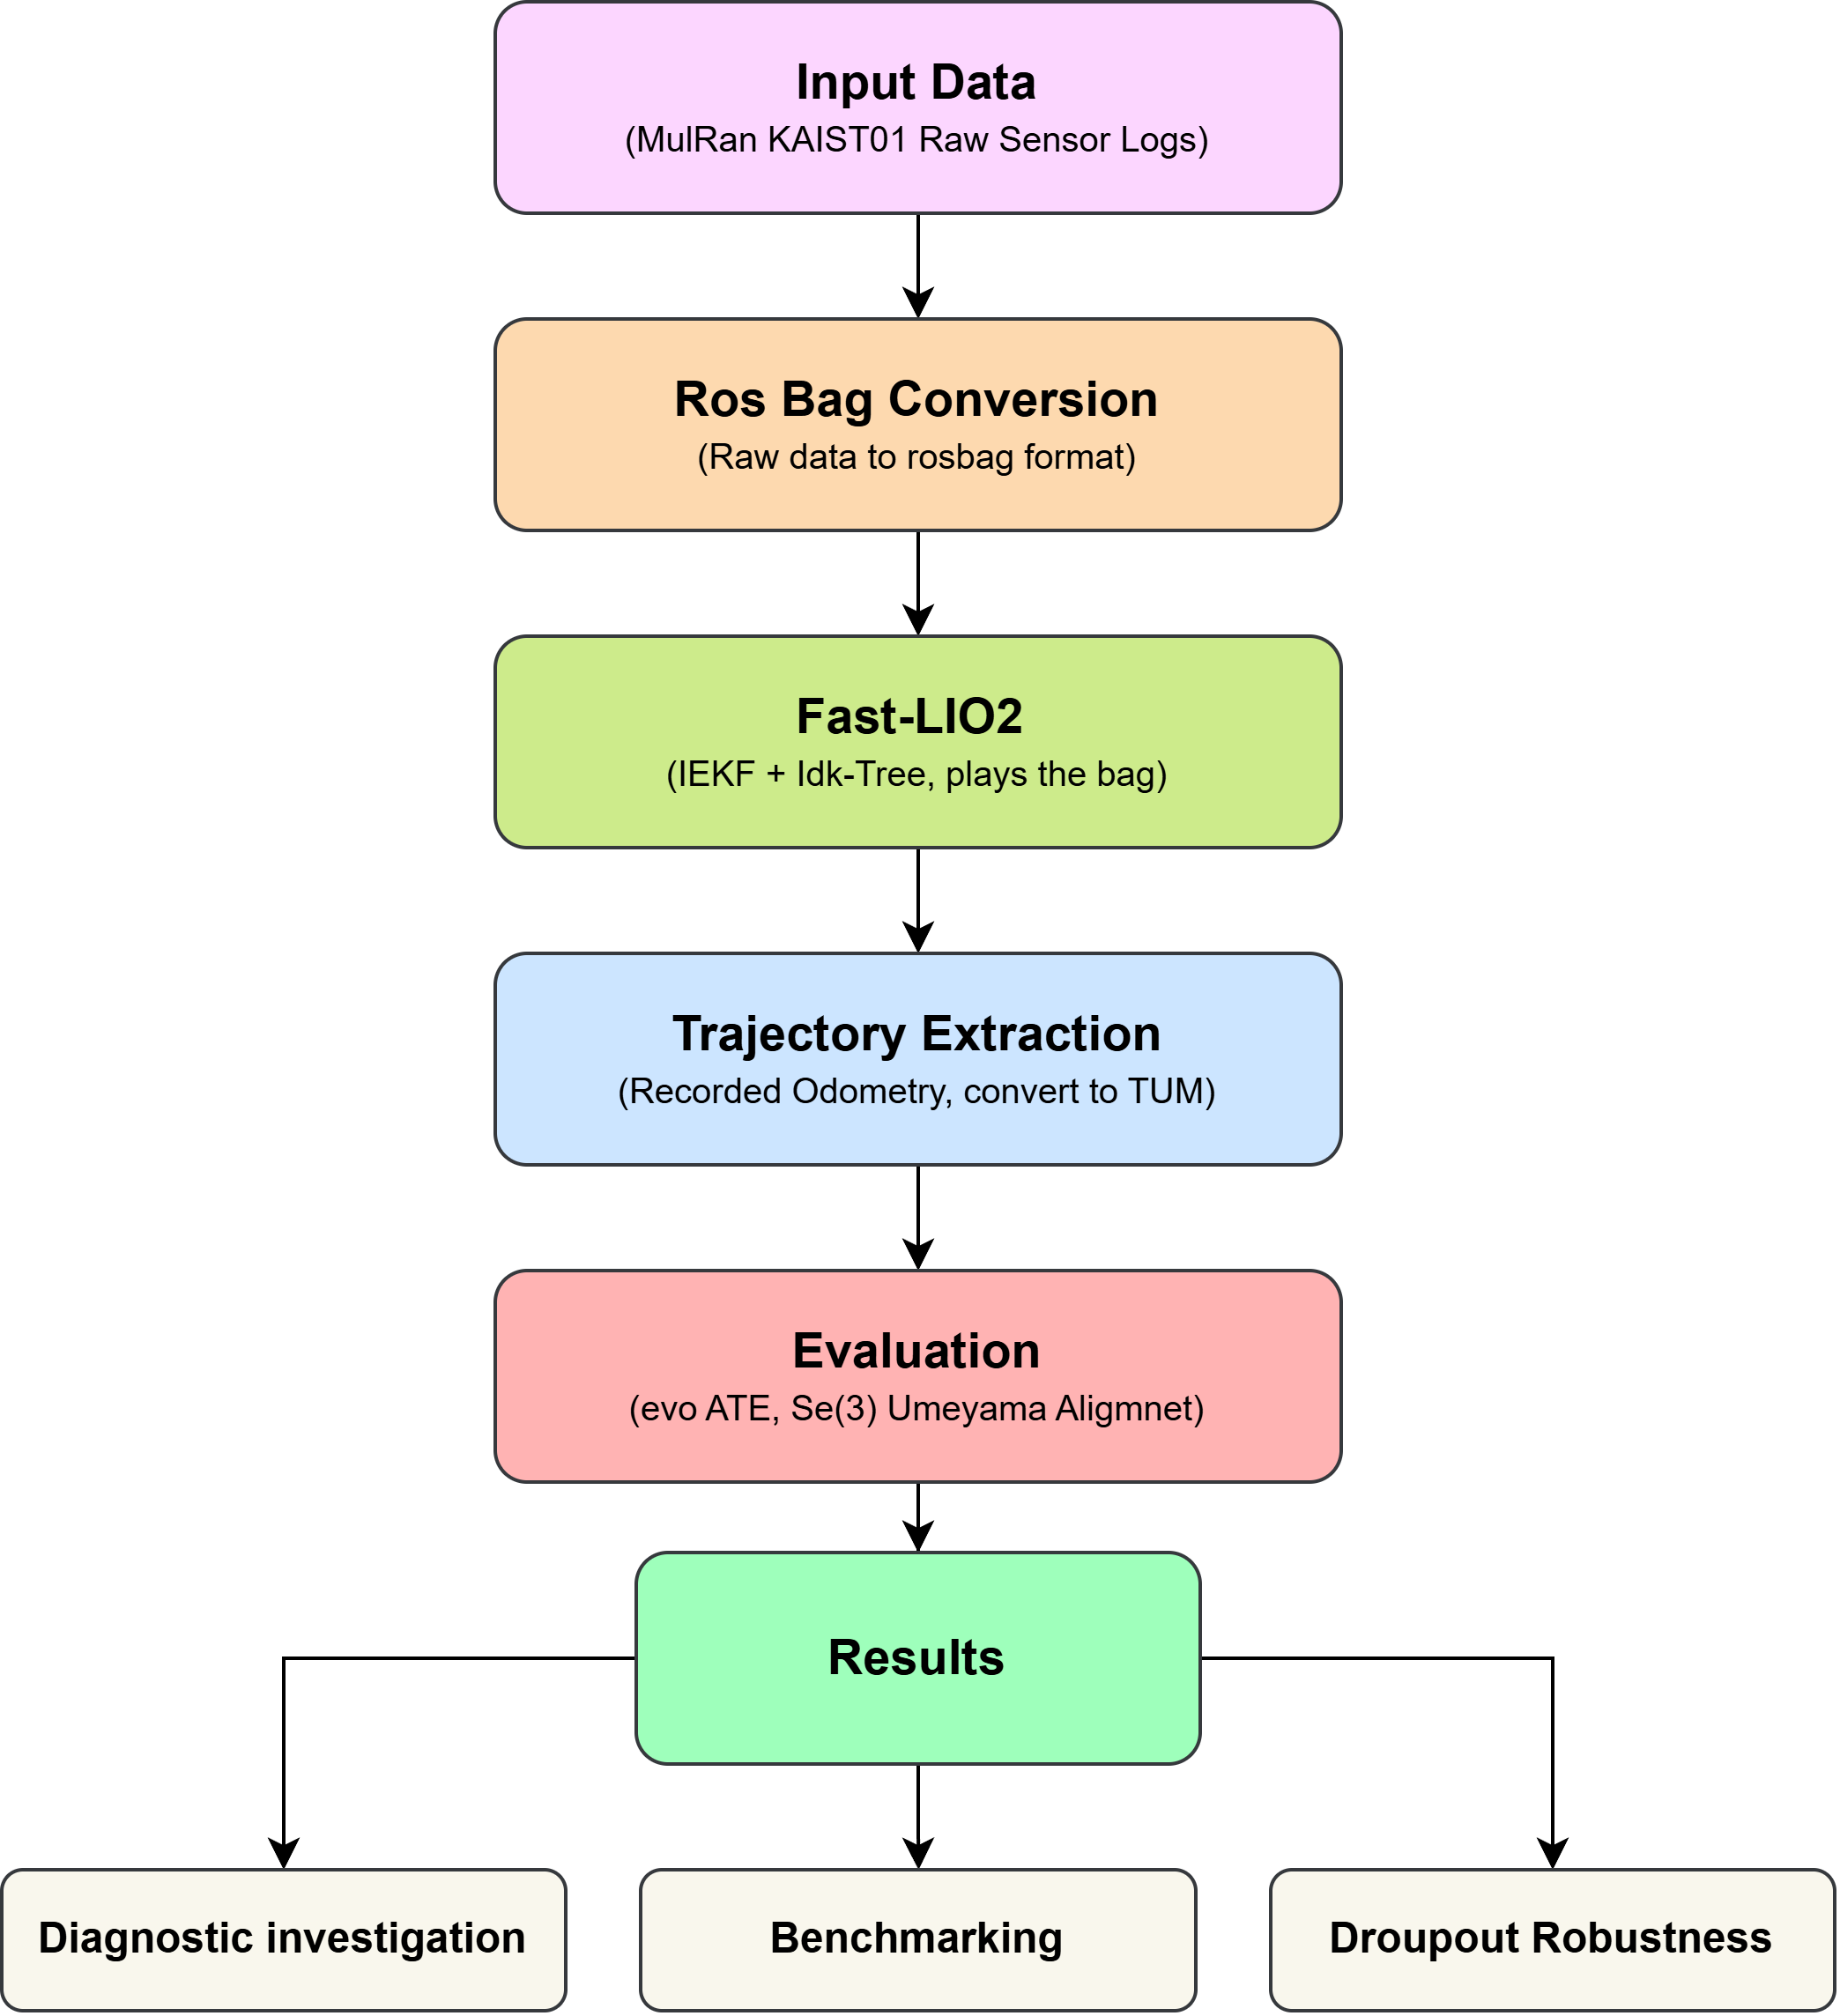
\includegraphics[width=0.85\columnwidth]{figures/System_Schmatic_drawio.png}
\caption{End-to-end pipeline: raw sensor logs $\rightarrow$ rosbag conversion $\rightarrow$ FAST-LIO2 $\rightarrow$ trajectory extraction $\rightarrow$ evaluation $\rightarrow$ downstream analyses.}
\label{fig:pipeline}
\end{figure}

Internally, FAST-LIO2 (Fig.~\ref{fig:internal}) fuses IMU angular velocity and acceleration through forward propagation to predict the state ahead of each incoming LiDAR scan. Raw LiDAR points (no feature extraction) are then registered against the ikd-Tree map through the iterated Kalman filter update, which jointly refines the state estimate (pose, velocity, sensor bias) and inserts newly observed points back into the map, re-balancing the tree as needed to keep query costs low.

\begin{figure}[htbp]
\centering
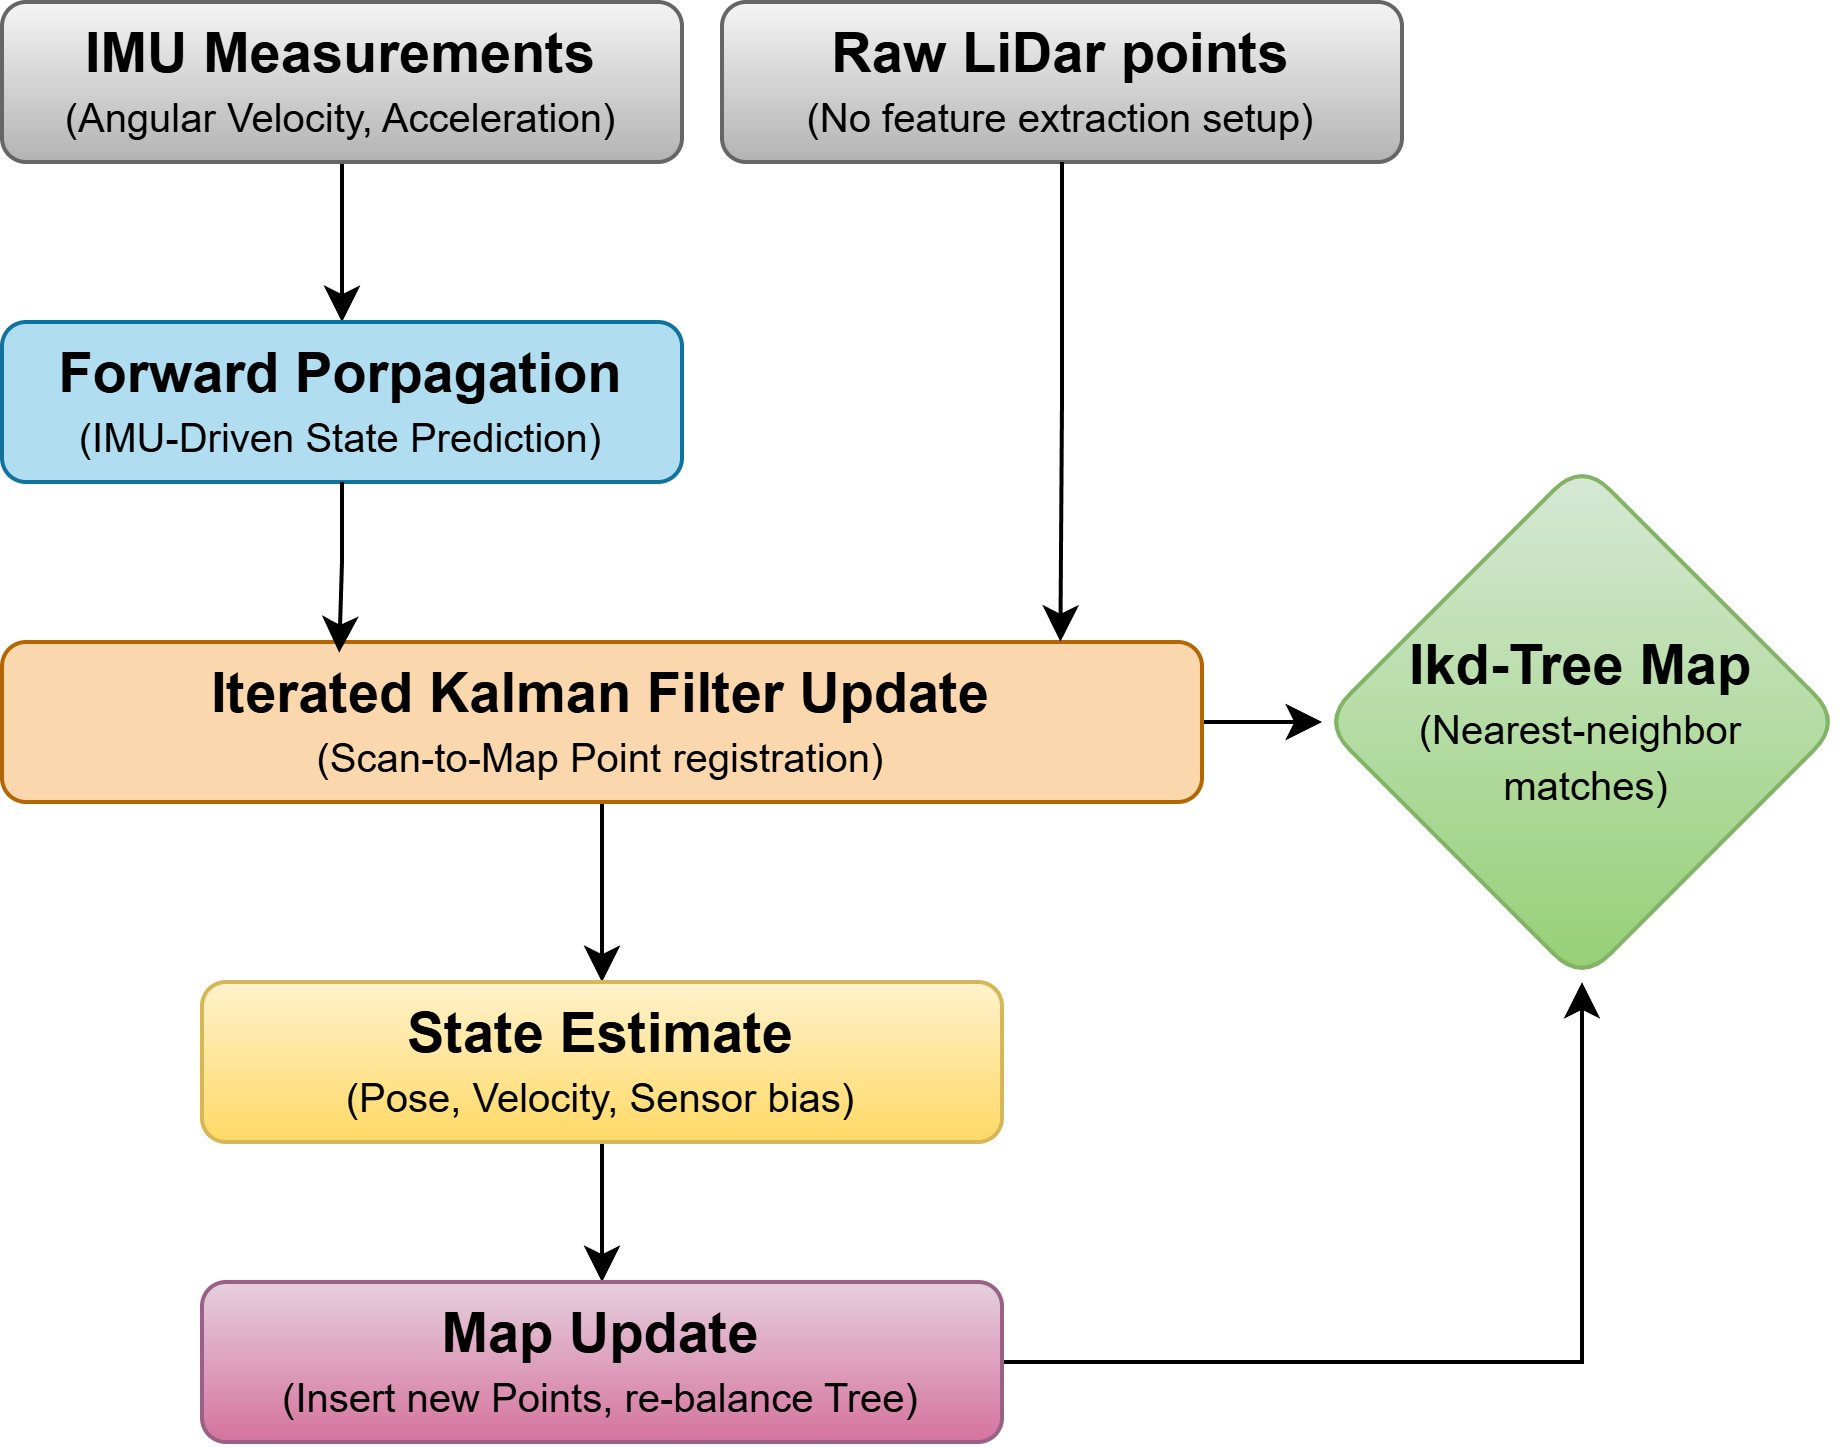
\includegraphics[width=\columnwidth]{figures/How_mapping_is_done_drawio.png}
\caption{FAST-LIO2 internal estimation loop: IMU forward propagation, iterated Kalman filter scan-to-map registration, and incremental ikd-Tree map maintenance.}
\label{fig:internal}
\end{figure}

\section{Experimental Setup}
All experiments were conducted on the platform and software configuration summarized in Table~\ref{tab:setup}.

\begin{table}[htbp]
\caption{System and Experimental Setup Summary}
\label{tab:setup}
\centering
\begin{tabular}{p{0.32\columnwidth}p{0.55\columnwidth}}
\toprule
\textbf{Parameter} & \textbf{Value} \\
\midrule
Platform & Lenovo Legion 5, WSL2 Ubuntu 20.04, ROS Noetic \\
Estimator & FAST-LIO2 (\texttt{ouster64.yaml} configuration) \\
Dataset & MulRan KAIST01 (Ouster OS1-64 LiDAR + Xsens IMU) \\
Driving distance & $\sim$863 m \\
Ground truth & \texttt{global\_pose.csv} --- 78,672 poses, UTM frame \\
Evaluation metric & ATE RMSE, evo \texttt{main\_ape}, SE(3) Umeyama alignment \\
\bottomrule
\end{tabular}
\end{table}

Before quantitative accuracy evaluation could be trusted, each stage of the data-processing chain was independently validated, since an unvalidated pipeline stage could masquerade as an estimator accuracy issue. Two implementation defects were identified and corrected during this process:

\begin{itemize}
\item \textbf{Trajectory recording:} initial recording via \texttt{rostopic echo -p} redirected to a file produced physically implausible z-excursions exceeding 1{,}000{,}000~m, because this method is lossy for high-rate topics. This was corrected by running \texttt{rosbag record} concurrently with playback and extracting the trajectory directly from the recorded bag via rosbag's Python API.
\item \textbf{IMU-to-bag conversion:} raw IMU CSV rows were compared directly against decoded ROS message values, revealing that \texttt{gyro.z} was reading $\sim$9.8--9.9 (the magnitude of gravity, not a plausible angular rate) and \texttt{linear\_acceleration} was a normalized unit vector rather than true acceleration --- the conversion script was reading the wrong CSV columns. Columns were corrected to match the documented MulRan \texttt{xsens\_imu.csv} layout (angular velocity in columns 8--10, linear acceleration in columns 11--13), after which position ranges (x: $-329.9$ to $313.8$~m, y: $-108.9$ to $654.1$~m, z: $-22.9$ to $100.3$~m) became physically realistic for the $\sim$863~m course.
\end{itemize}

With these two corrections in place and independently verified, the pipeline was considered validated and ready for quantitative accuracy evaluation, presented in Section~\ref{sec:results}.

\section{Results and Discussion}
\label{sec:results}

\subsection{Measured Accuracy and Diagnostic Investigation}
\label{sec:diag}
Following pipeline validation, the measured localization accuracy was 30.19~m ATE RMSE, with evo's Umeyama alignment consistently reporting an approximately 68\textdegree{} rotational offset between the estimated and ground-truth trajectories. This 30.19~m figure corresponds specifically to the ``Test A'' configuration (identity extrinsic with online estimation enabled, \texttt{extrinsic\_est\_en: true}) introduced in Table~\ref{tab:extrinsic} below; this configuration was adopted as the pipeline's default for all downstream analysis in this report, including the benchmarking in Section~\ref{sec:benchmark} and the dropout robustness sweep in Section~\ref{sec:extensions}, and should be distinguished from the 30.34~m ``Baseline (original)'' row of Table~\ref{tab:extrinsic}, which used a fixed identity extrinsic with online estimation disabled. Because a rotational alignment offset of this size could plausibly arise from LiDAR-IMU extrinsic miscalibration or from a coordinate-frame/axis-convention mismatch, both hypotheses were investigated systematically, following a specific concern raised in supervisor feedback that the offset was unlikely to be explained by extrinsic calibration alone.

The ground-truth conversion pipeline was independently validated line-by-line --- the rotation-matrix-to-quaternion conversion (Shepperd's method) and the row indexing used to build the TUM-format ground truth were checked against the documented 13-column layout of \texttt{global\_pose.csv} and confirmed correct, ruling this out as a contributing factor. Raw IMU data was likewise read directly from the bag to verify sign convention and axis orientation at the source: angular velocity was near-zero at rest (x~=~$-0.0014$, y~=~$0.0005$, z~=~$-0.0026$~rad/s) and linear acceleration showed gravity on the $+Z$ axis (x~=~$-0.104$, y~=~$0.120$, z~=~$9.913$~m/s\textsuperscript{2}), consistent with a standard ENU / REP-103 convention, and frame IDs (IMU: ``imu'', LiDAR: ``os\_sensor'') were confirmed sane --- ruling out raw IMU sign inversion as a factor.

With ground truth and raw IMU signs validated, three independent LiDAR-IMU extrinsic configurations were experimentally evaluated, each re-run through the complete pipeline (roscore $\rightarrow$ FAST-LIO2 $\rightarrow$ rosbag record $\rightarrow$ trajectory extraction $\rightarrow$ evo ATE) under otherwise identical conditions, summarized in Table~\ref{tab:extrinsic}.

\begin{table}[htbp]
\caption{Extrinsic-Calibration Experiment Configurations and Results}
\label{tab:extrinsic}
\centering
\begin{tabular}{p{0.19\columnwidth}p{0.19\columnwidth}p{0.13\columnwidth}p{0.1\columnwidth}p{0.16\columnwidth}}
\toprule
\textbf{Config.} & \textbf{extrinsic\_R} & \textbf{est.\ en.} & \textbf{RMSE (m)} & \textbf{Umeyama rot.} \\
\midrule
Baseline (original) & Identity & false & 30.34 & $\sim$68\textdegree{} about Z \\
Test A --- Online est. & Identity (init.) & true & 30.19 & $\sim$68\textdegree{} about Z \\
Test B --- 180\textdegree{} about Z & $[-1,0,0;\allowbreak 0,-1,0;\allowbreak 0,0,1]$ & true & 39.95 & $\sim{-}68$\textdegree{} (mirrored) \\
\bottomrule
\end{tabular}
\end{table}

Test A enabled FAST-LIO2's online extrinsic refinement, starting from an identity initial value, allowing the filter to estimate a better LiDAR-IMU rotation/translation automatically. This produced RMSE~=~30.19~m, closely matching the 30.34~m baseline, with the Umeyama rotation still reporting $\sim$68\textdegree, indicating online estimation did not meaningfully change the measured accuracy.

\begin{figure}[htbp]
\centering
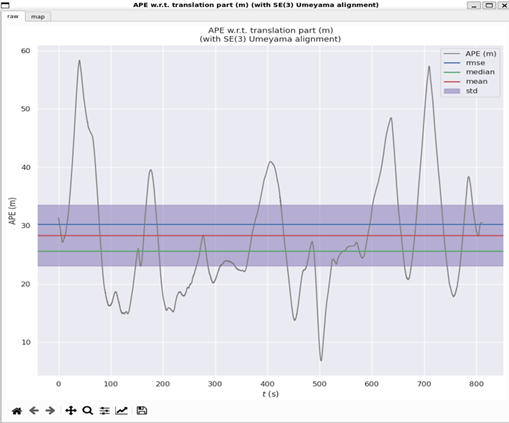
\includegraphics[width=0.85\columnwidth]{figures/Ape_vs_Time_-_Test_A.png}
\caption{APE vs.\ time --- Test A (online extrinsic estimation, identity initial value). RMSE = 30.19~m.}
\label{fig:apeA}
\end{figure}

\begin{figure}[htbp]
\centering
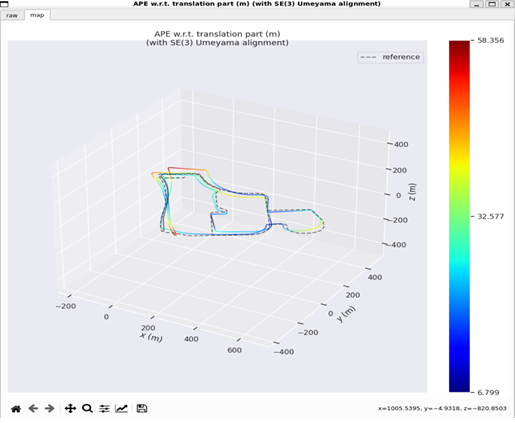
\includegraphics[width=0.85\columnwidth]{figures/3d_Trajactory_-_Test_A.png}
\caption{3D trajectory comparison --- Test A. Estimated path (colour = error) vs.\ ground truth (dashed).}
\label{fig:trajA}
\end{figure}

Test B set \texttt{extrinsic\_R} to a 180\textdegree{} rotation about the vertical (Z) axis --- representing a scenario where the IMU is mounted facing the opposite horizontal direction to the LiDAR --- as a targeted, physically plausible hypothesis test. This produced RMSE~=~39.95~m, higher than both the baseline and Test A, ruling out a simple 180\textdegree{} yaw mounting offset as the explanation.

\begin{figure}[htbp]
\centering
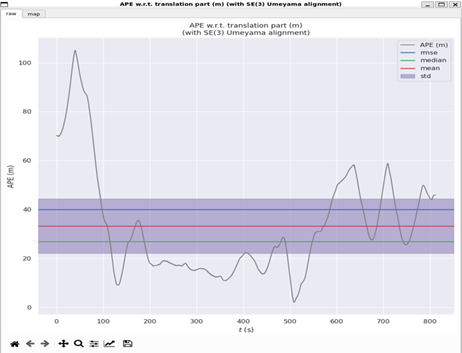
\includegraphics[width=0.85\columnwidth]{figures/Ape_vs_Time_-_Test_B.png}
\caption{APE vs.\ time --- Test B (180\textdegree{} about Z). RMSE = 39.95~m.}
\label{fig:apeB}
\end{figure}

\begin{figure}[htbp]
\centering
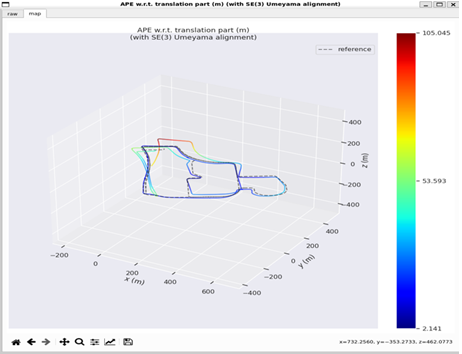
\includegraphics[width=0.85\columnwidth]{figures/3d_Trajactory_-_Test_B.png}
\caption{3D trajectory comparison --- Test B.}
\label{fig:trajB}
\end{figure}

Two observations follow from this pattern: first, measured RMSE does not respond substantially to changes in the extrinsic value, including online estimation, suggesting the extrinsic value alone is unlikely to be the dominant factor governing accuracy in this configuration; second, the APE-vs-time behavior in both tests (Figs.~\ref{fig:apeA}, \ref{fig:apeB}) shows the error present from the very start of the run rather than growing steadily, a pattern more typically associated with a systematic effect than with accumulated drift. Together with the validated ground-truth pipeline and raw IMU signs, the experimental evidence points toward a systematic frame- or axis-related effect --- consistent with the professor's hypothesis of an Ouster-versus-REP-103 axis-convention mismatch --- as the leading explanation, though further frame-level analysis (TF-tree inspection, explicit axis-convention verification) would be required for definitive confirmation. Fig.~\ref{fig:diagnosis} summarizes this diagnostic workflow.

\begin{figure}[htbp]
\centering
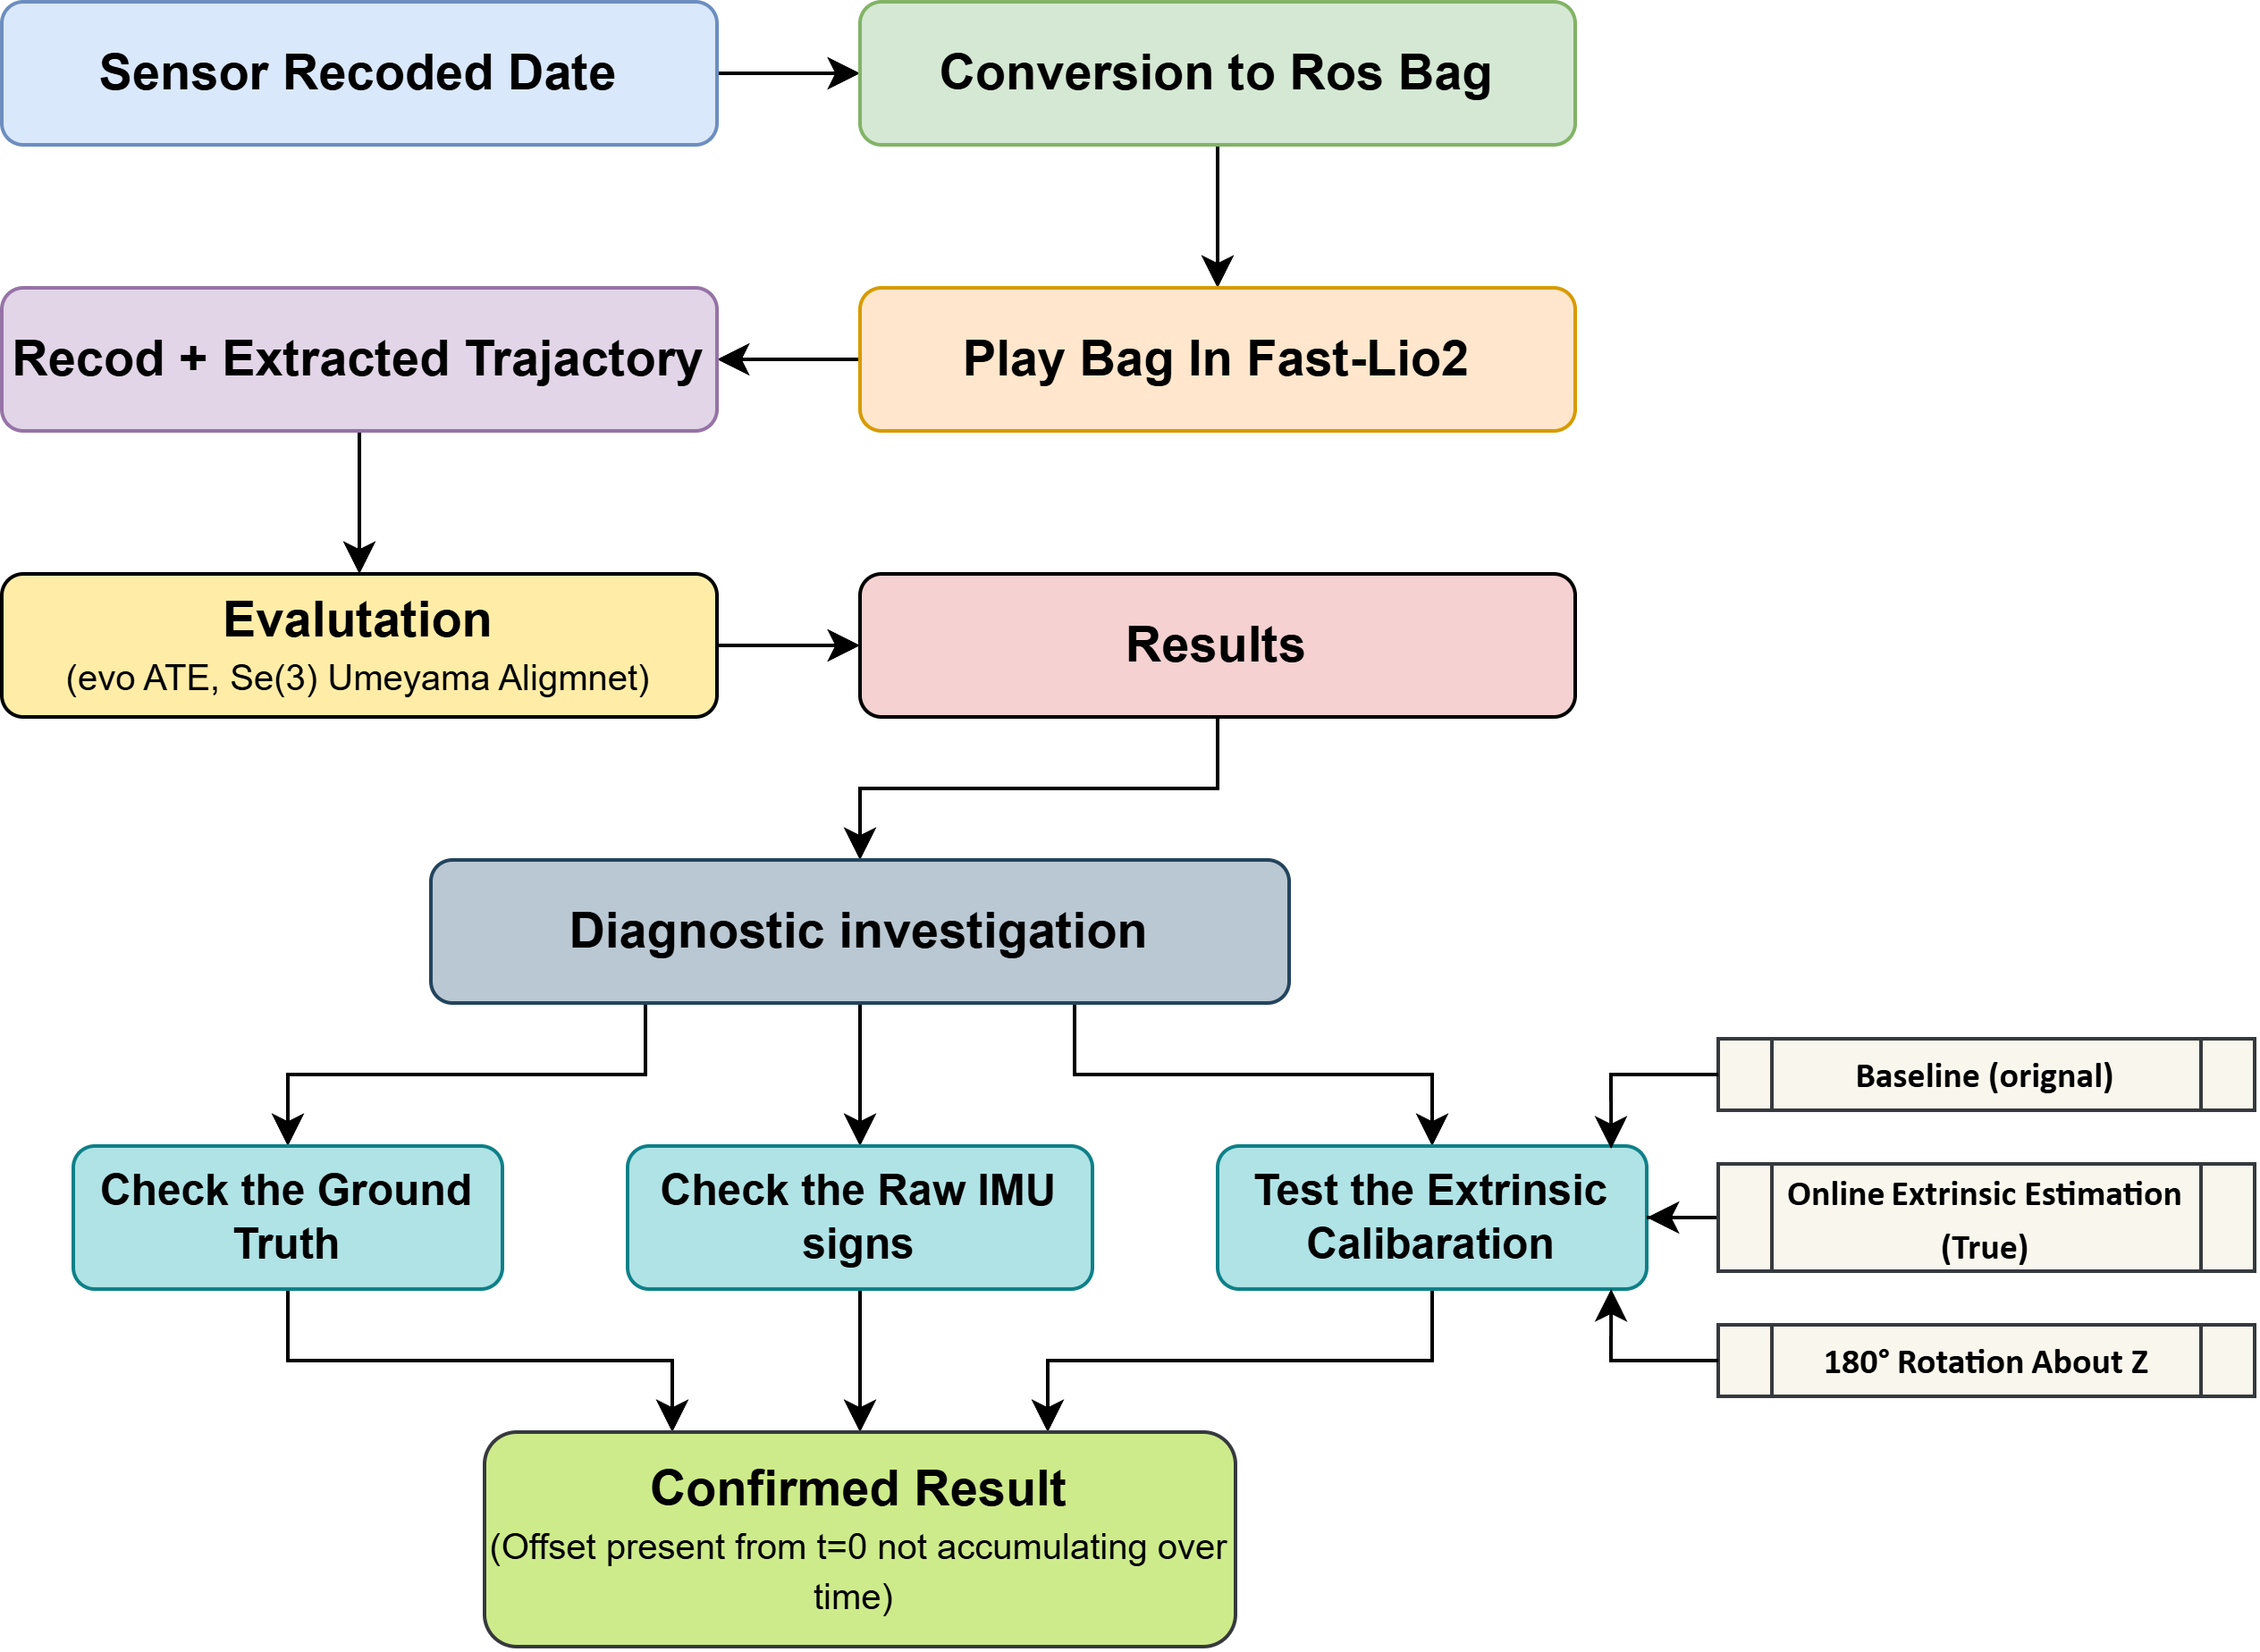
\includegraphics[width=\columnwidth]{figures/Diagonosis_drawio.png}
\caption{Diagnostic investigation workflow: ground-truth, raw IMU, and extrinsic-calibration validation converging on a confirmed offset present from $t=0$ rather than accumulating over time.}
\label{fig:diagnosis}
\end{figure}

The rotational component was also cross-checked numerically from the Umeyama alignment output:
\begin{equation}
\mathrm{tr}(R) = 0.365 + 0.364 + 0.994 = 1.723
\label{eq:trace}
\end{equation}
\begin{equation}
\cos\theta = \frac{\mathrm{tr}(R) - 1}{2} = 0.362
\label{eq:costheta}
\end{equation}
\begin{equation}
\theta = \arccos(0.362) \approx 68.8\text{\textdegree}
\label{eq:theta}
\end{equation}
The remarkable consistency of this $\sim$68\textdegree{} figure across all three tested extrinsic configurations is treated here as a secondary, exploratory diagnostic finding --- a preliminary result and known limitation of this reproduction rather than a resolved conclusion, in keeping with the emphasis on honest critical analysis over simple reproduction claims.

\subsection{Benchmarking Against Published Results}
\label{sec:benchmark}
To place the measured accuracy in context, it was compared against published FAST-LIO2 results on comparable large-scale outdoor driving sequences (Table~\ref{tab:benchmark}), rather than against short indoor/handheld tests that are not representative of this scenario.

\begin{table}[htbp]
\caption{Benchmarking Against Published FAST-LIO2 Results}
\label{tab:benchmark}
\centering
\begin{tabular}{p{0.62\columnwidth}p{0.24\columnwidth}}
\toprule
\textbf{Source / Sequence} & \textbf{RMSE} \\
\midrule
FAST-LIO2 paper --- utbm\_8 (outdoor driving) & 25.3 m \\
FAST-LIO2 paper --- utbm\_9 (outdoor driving) & 51.6 m \\
FAST-LIO2 paper --- utbm\_10 (outdoor driving) & 16.9 m \\
FAST-LIO2 + Scan Context loop closure --- MulRan DCC01 & 7.58 m \\
This work --- MulRan KAIST01 (no loop closure) & 30.19 m \\
\bottomrule
\end{tabular}
\end{table}

The measured 30.19~m RMSE lies within the 17--52~m range reported for comparable outdoor driving sequences, indicating the achieved accuracy is consistent with previously published results for this class of scenario rather than an anomalous deviation. The MulRan DCC01 result of 7.58~m was achieved with Scan Context loop-closure correction layered on top of FAST-LIO2, whereas this project evaluates FAST-LIO2 alone as pure odometry with no loop closure, since the algorithm as released includes no loop-detection module --- some additional drift relative to a loop-closure-corrected system is therefore expected. It is important to distinguish two related but separate findings: localization accuracy (benchmarked here as consistent with the literature) and the alignment observation from Section~\ref{sec:diag} (a separate, exploratory diagnostic finding warranting continued investigation independent of this benchmarking result).

\section{Extensions Beyond Original Work}
\label{sec:extensions}
As the primary research extension of this project, and after establishing a validated baseline (Sections IV--VI), the work was extended with a controlled synthetic point-cloud dropout study to independently evaluate how localization accuracy responds to degraded LiDAR sensing --- a proxy for real-world conditions such as fog, rain, or dust, where a fraction of LiDAR returns are lost to scattering or absorption rather than reaching a solid surface and returning cleanly.

\subsection{Method}
Rather than sourcing a separate real fog/rain dataset --- which would require an entirely new sensor platform, calibration, and ground-truth pipeline --- a synthetic dropout framework (Fig.~\ref{fig:dropoutmethod}) was designed and applied directly to the existing, validated KAIST01 bag. For each LiDAR scan, a specified percentage of points was randomly removed before being written to a new bag. The same dataset, IMU stream, FAST-LIO2 configuration, and evaluation pipeline were preserved throughout, isolating point-cloud density as the single varied factor. Four dropout levels were tested --- 10\%, 30\%, 50\%, and 70\% of points removed per scan --- in addition to the 0\% baseline, each run through the identical roscore $\rightarrow$ FAST-LIO2 $\rightarrow$ rosbag record $\rightarrow$ evo ATE pipeline, using the best-performing configuration identified in Section~\ref{sec:diag} (identity extrinsic with online estimation enabled).

\begin{figure}[htbp]
\centering
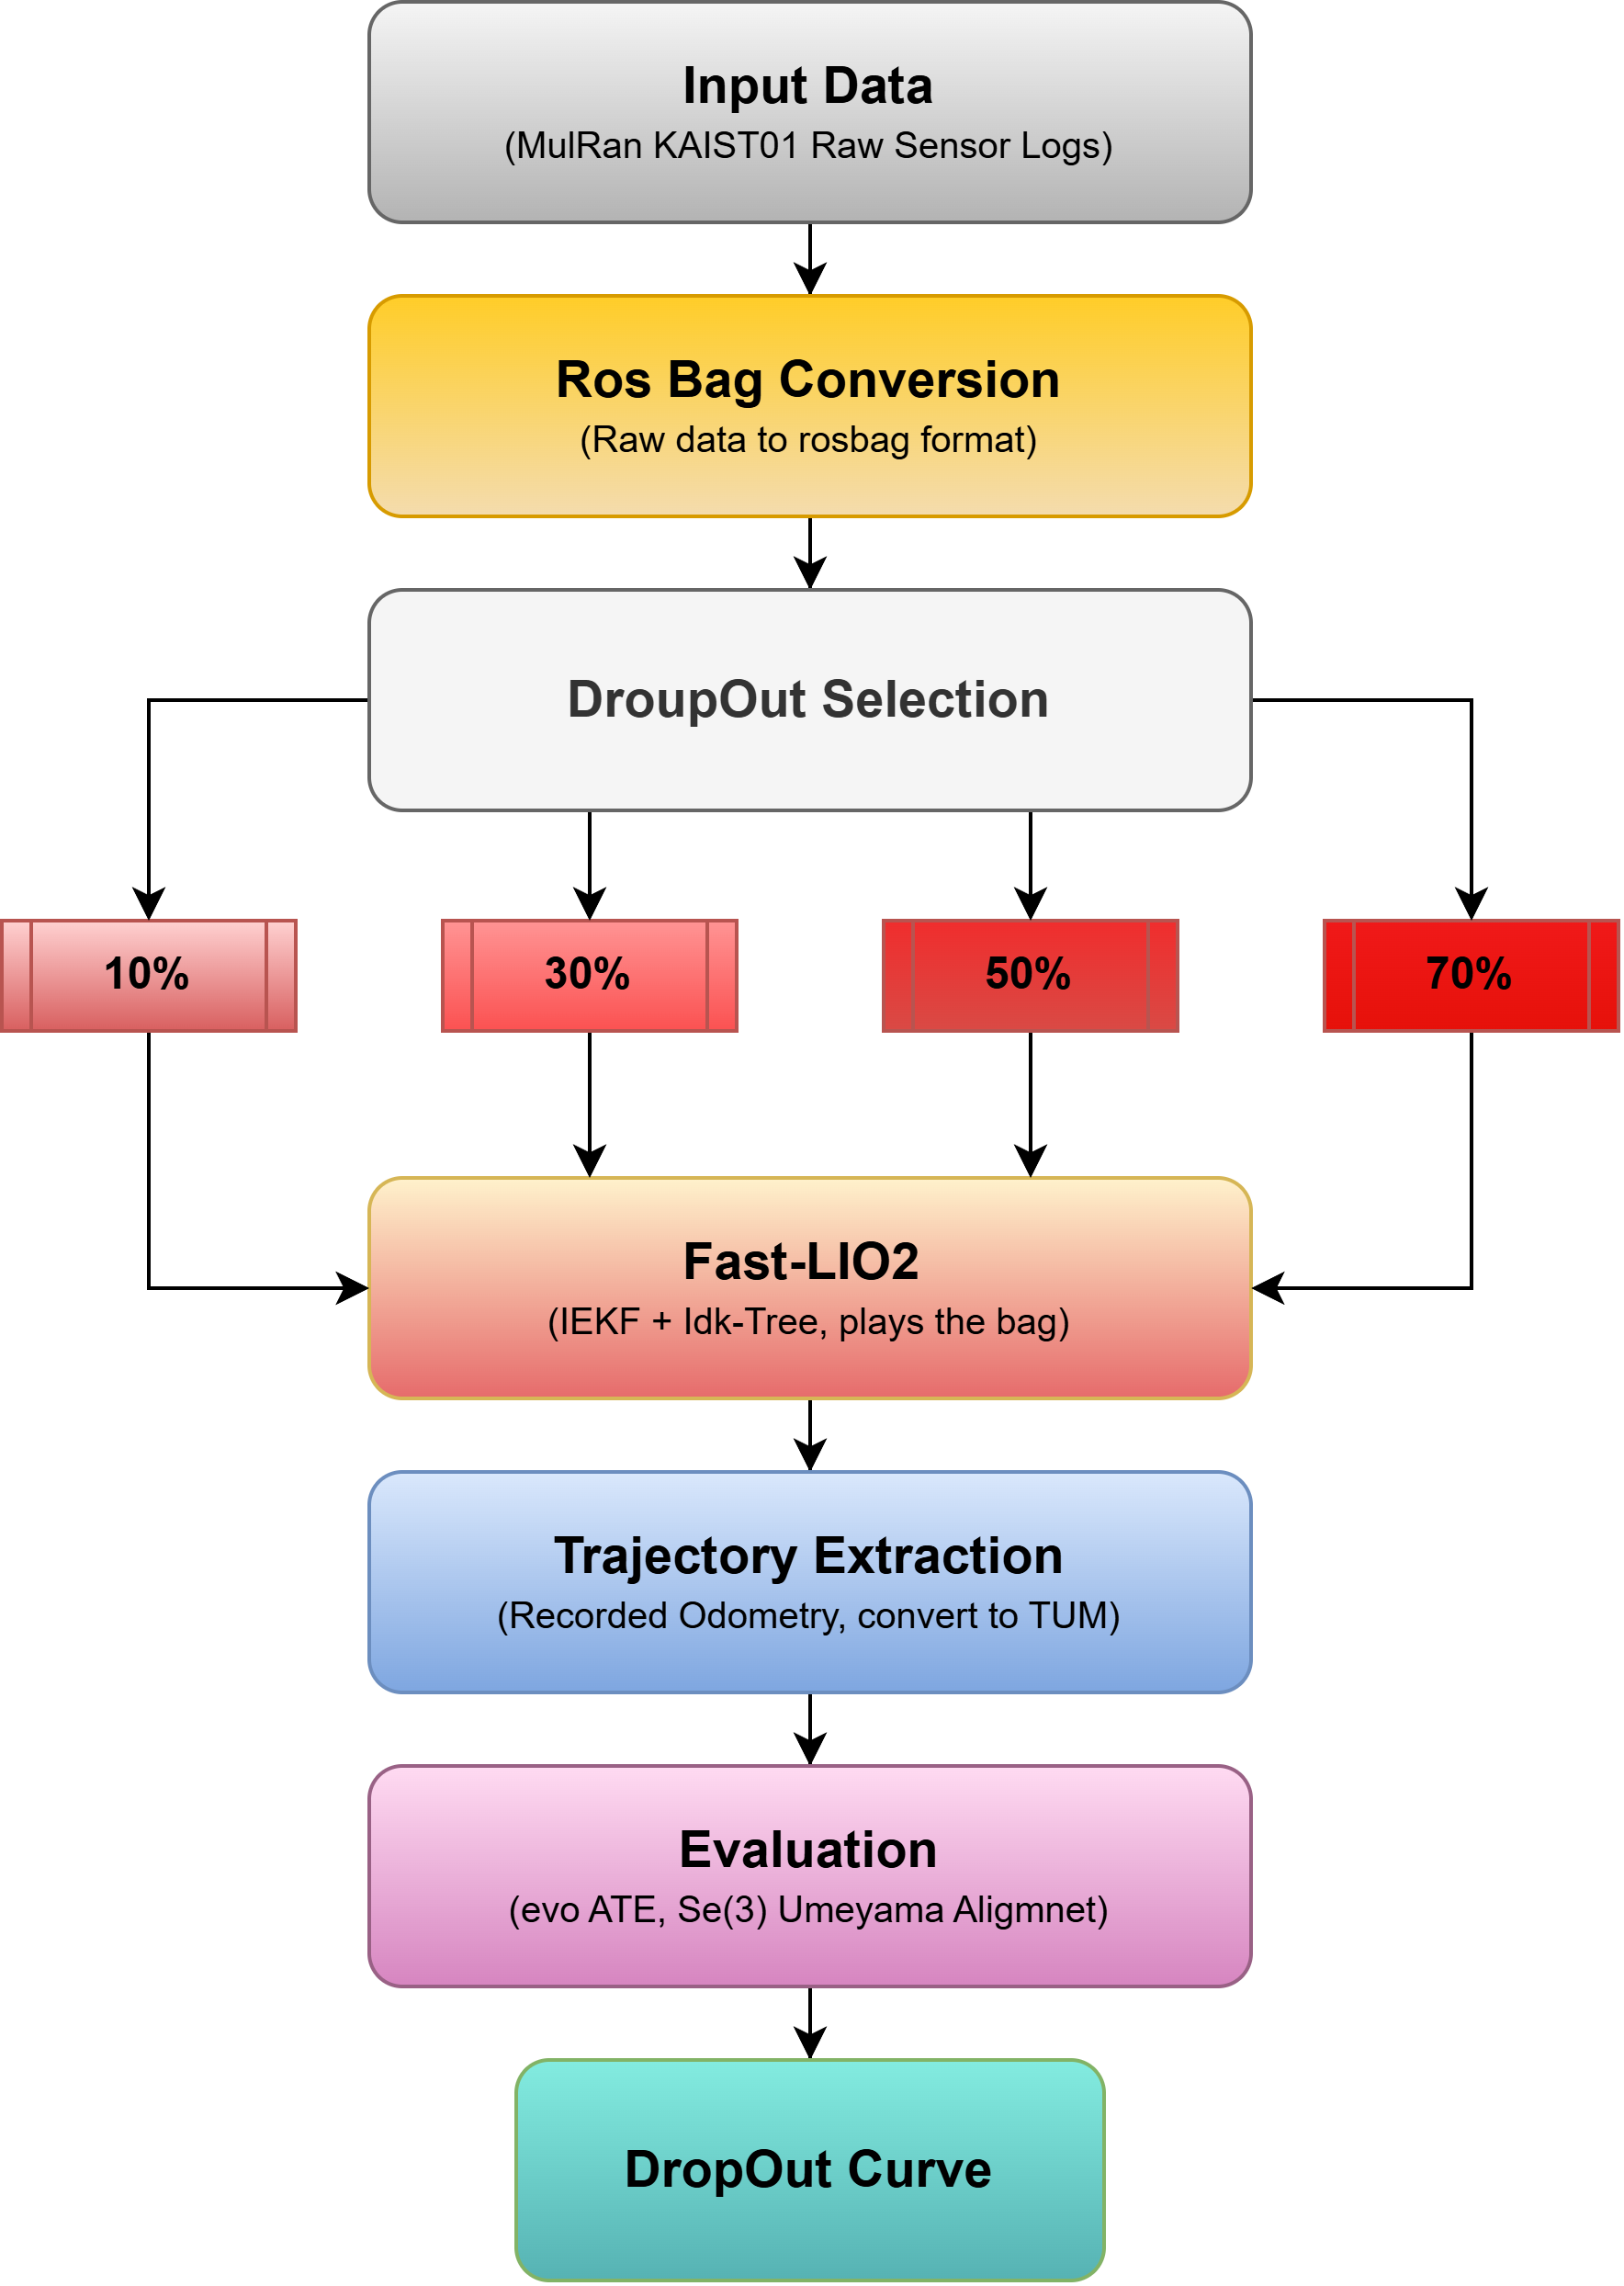
\includegraphics[width=0.72\columnwidth]{figures/DropOut_selection_drawio.png}
\caption{Point-cloud dropout evaluation pipeline: dataset routed through 10/30/50/70\% dropout selection before FAST-LIO2, trajectory extraction, and evaluation.}
\label{fig:dropoutmethod}
\end{figure}

\subsection{Results}

\begin{figure}[htbp]
\centering
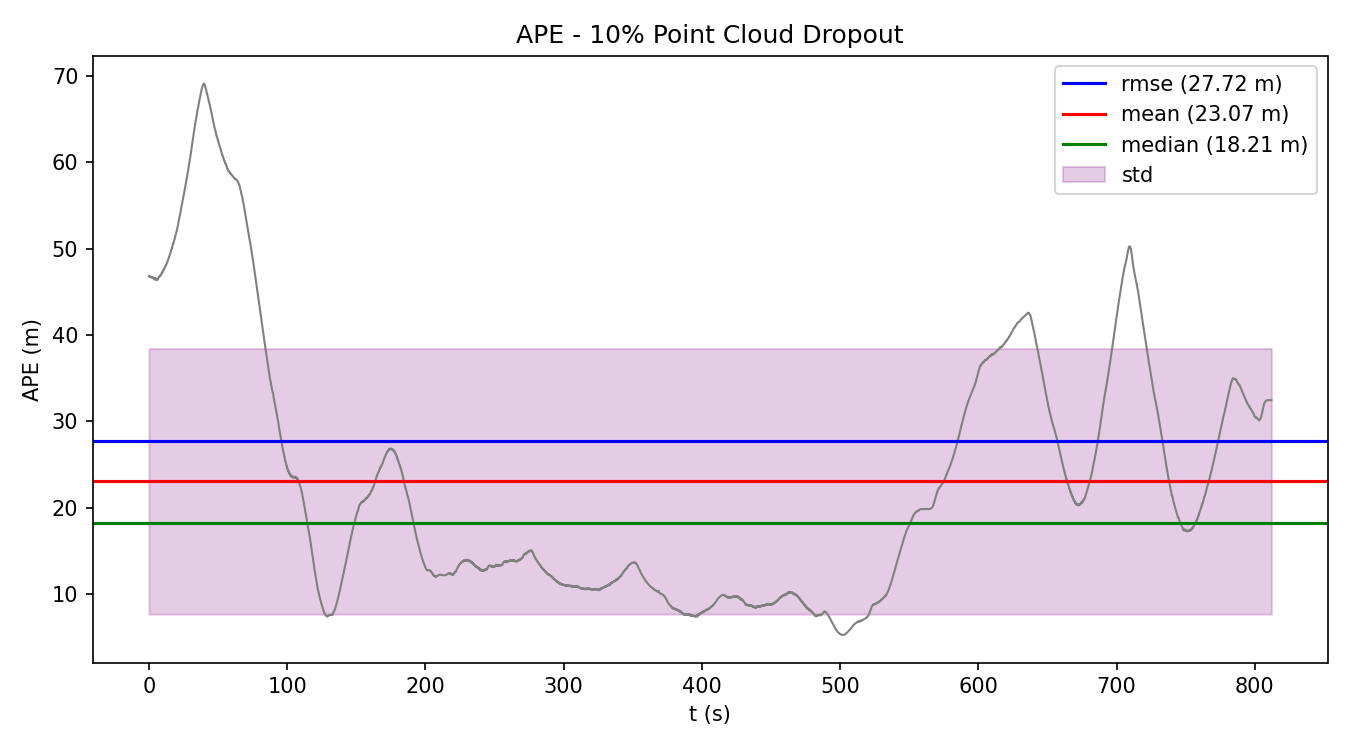
\includegraphics[width=0.85\columnwidth]{figures/plot_dropout10.png}
\caption{APE vs.\ time --- 10\% dropout. RMSE = 27.72~m.}
\label{fig:d10}
\end{figure}

\begin{figure}[htbp]
\centering
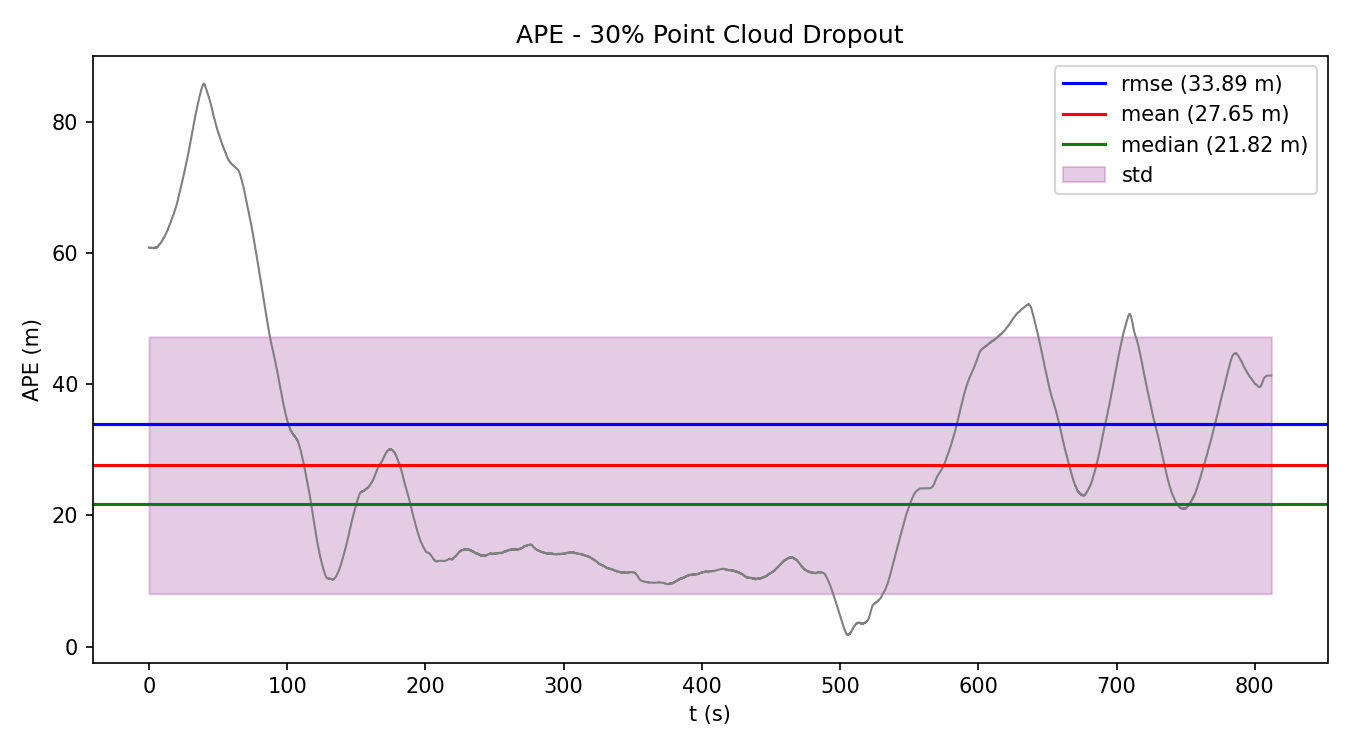
\includegraphics[width=0.85\columnwidth]{figures/plot_dropout30.png}
\caption{APE vs.\ time --- 30\% dropout. RMSE = 33.89~m.}
\label{fig:d30}
\end{figure}

\begin{figure}[htbp]
\centering
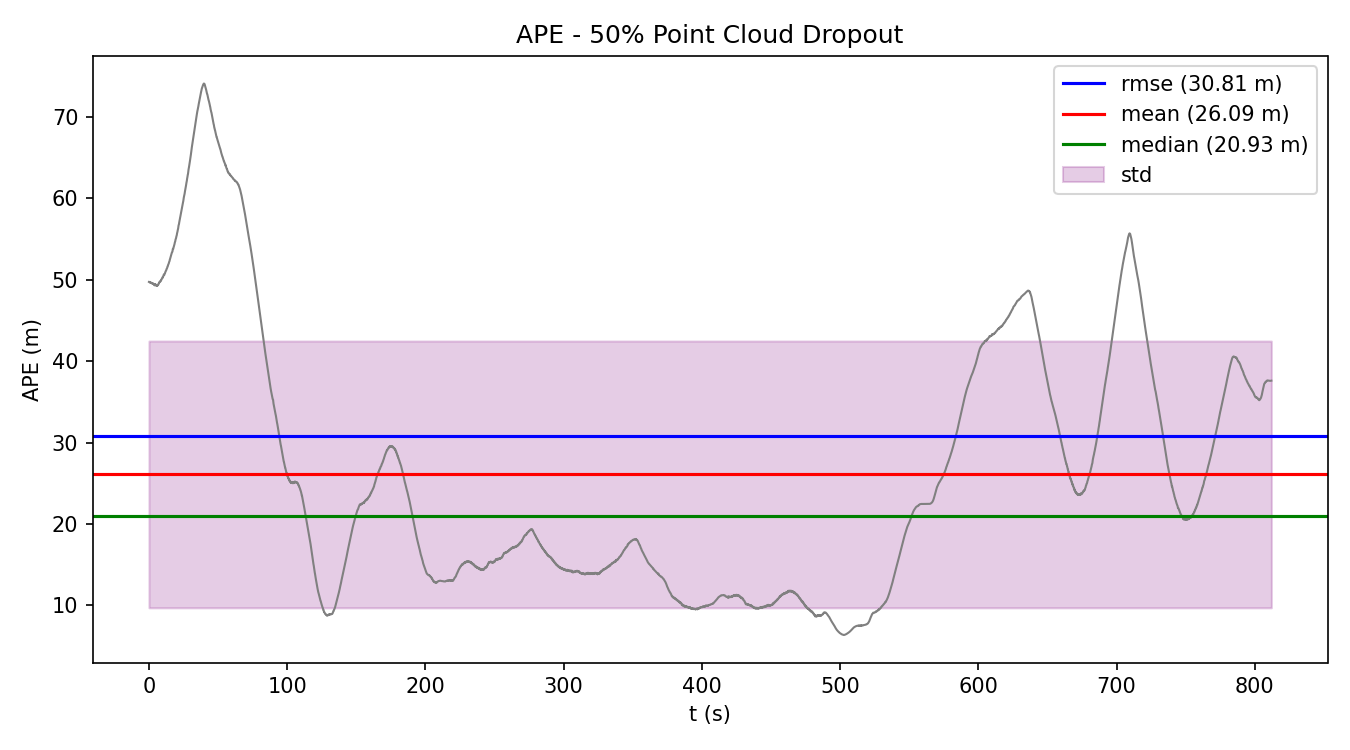
\includegraphics[width=0.85\columnwidth]{figures/plot_dropout50.png}
\caption{APE vs.\ time --- 50\% dropout. RMSE = 30.81~m.}
\label{fig:d50}
\end{figure}

\begin{figure}[htbp]
\centering
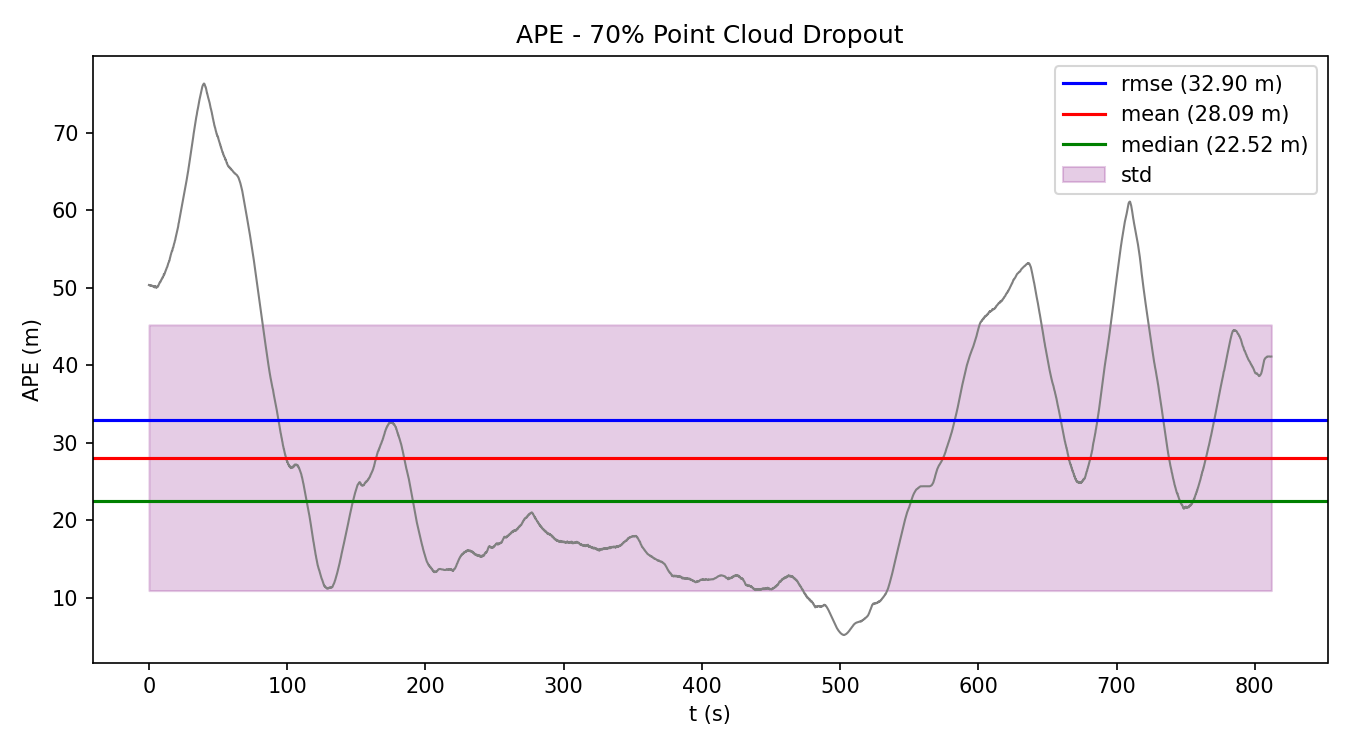
\includegraphics[width=0.85\columnwidth]{figures/plot_dropout70.png}
\caption{APE vs.\ time --- 70\% dropout. RMSE = 32.90~m.}
\label{fig:d70}
\end{figure}

\begin{table}[htbp]
\caption{ATE RMSE Across the Point-Cloud Dropout Sweep}
\label{tab:dropout}
\centering
\begin{tabular}{p{0.4\columnwidth}p{0.4\columnwidth}}
\toprule
\textbf{Dropout Level} & \textbf{RMSE (m)} \\
\midrule
0\% (baseline) & 30.19 \\
10\% & 27.72 \\
30\% & 33.89 \\
50\% & 30.81 \\
70\% & 32.90 \\
\bottomrule
\end{tabular}
\end{table}

\begin{figure}[htbp]
\centering
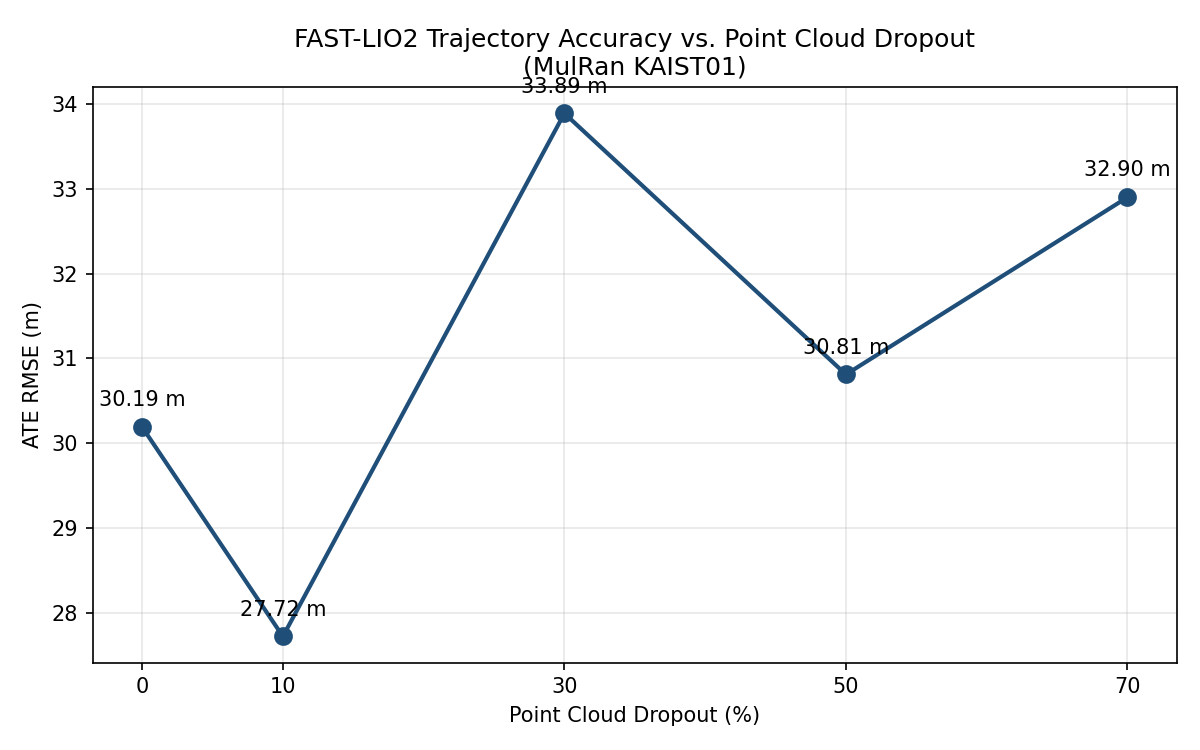
\includegraphics[width=\columnwidth]{figures/plot_dropout_summary.png}
\caption{ATE RMSE as a function of point-cloud dropout percentage, 0--70\%.}
\label{fig:dropoutsummary}
\end{figure}

\subsection{Interpretation}
Across the full 0--70\% dropout range, RMSE remains within a comparatively narrow band (27.7--33.9~m) with no clear monotonic degradation trend --- the value moves up and down rather than increasing steadily with dropout, and even the most heavily degraded case (70\%) remains close to the clean baseline. This is a meaningful result in its own right: localization accuracy remained stable across a wide range of synthetic LiDAR degradation, indicating a useful degree of robustness in the implementation under the tested conditions. If localization accuracy were primarily driven by sensitivity to point-cloud density, RMSE would be expected to climb steadily as more points are removed; instead it stays anchored around a similar level regardless of how much of the point cloud is discarded, suggesting point-cloud density alone is unlikely to explain the measured accuracy.

Two factors likely contribute to the absence of a clean monotonic trend. First, whatever systematic effect underlies the baseline RMSE (Section~\ref{sec:diag}) appears to be a larger contributor than point-cloud density on its own, making any smaller density-dependent effect difficult to isolate against that background level. Second, FAST-LIO2's scan-matching front end is inherently somewhat tolerant of moderate point loss by design --- it requires sufficient scan-to-scan overlap rather than every point converging --- so dropout in the 10--50\% range is not necessarily severe enough to push the estimator into a distinct failure mode. A natural follow-up would be to repeat this sweep once the alignment observation of Section~\ref{sec:diag} is further characterized, to check whether a clearer density-dependent trend emerges under more tightly controlled conditions.

\section{Comparison with Original Paper}
Tables~\ref{tab:comparison1} and \ref{tab:comparison2} summarize, respectively, how this reproduction compares feature-by-feature against the original FAST-LIO2 paper, and how each extension carried out in this work relates to its motivation and outcome.

\begin{table}[htbp]
\caption{Feature-by-Feature Comparison with the Original FAST-LIO2 Paper}
\label{tab:comparison1}
\centering
\begin{tabular}{p{0.22\columnwidth}p{0.32\columnwidth}p{0.30\columnwidth}}
\toprule
\textbf{Feature} & \textbf{Original Paper \cite{fastlio2}} & \textbf{This Work} \\
\midrule
Robot Platform & UAV, handheld device, ground vehicle (multiple platforms) & Ground vehicle (MulRan KAIST01 recording platform) \\
Environment & Indoor, handheld, and outdoor driving sequences & Large-scale outdoor urban driving ($\sim$863 m) \\
Sensors & Various LiDAR models + IMU (platform-dependent) & Ouster OS1-64 LiDAR + Xsens IMU \\
Algorithm & FAST-LIO2 (iEKF + ikd-Tree, no loop closure) & FAST-LIO2 (\texttt{ouster64.yaml}), unmodified estimator \\
Evaluation Scenarios & Multiple public/self-collected datasets, incl.\ short outdoor driving & Single large-scale outdoor sequence, KAIST01 \\
Performance Metrics & ATE RMSE (varies by sequence) & ATE RMSE, SE(3) Umeyama alignment (evo) \\
Results & $\sim$17--52 m RMSE on comparable outdoor driving sequences & 30.19 m RMSE (within published range) \\
Limitations & No loop closure; sensitivity to extrinsic/frame handling not deeply studied & Same, plus an unresolved $\sim$68\textdegree{} alignment offset flagged as a preliminary finding \\
\bottomrule
\end{tabular}
\end{table}

\begin{table}[htbp]
\caption{Summary of Extensions, Motivation, and Outcomes}
\label{tab:comparison2}
\centering
\begin{tabular}{p{0.28\columnwidth}p{0.28\columnwidth}p{0.28\columnwidth}}
\toprule
\textbf{Extension} & \textbf{Motivation} & \textbf{Outcome} \\
\midrule
Diagnostic extrinsic-calibration study (3 configurations) & Supervisor feedback questioned whether the $\sim$68\textdegree{} alignment offset could be explained by LiDAR-IMU extrinsic miscalibration & Extrinsic value shown to have minimal effect on RMSE/rotation; a frame/axis-convention effect is the leading remaining hypothesis \\
Point-cloud dropout robustness sweep (0--70\%) & Original paper does not evaluate robustness to degraded sensing; motivated by real-world fog/rain/dust conditions & RMSE stable within a $\sim$6 m band across all dropout levels, indicating robustness to point-cloud density reduction \\
\bottomrule
\end{tabular}
\end{table}

\section{Challenges and Lessons Learned}

\begin{itemize}
\item \textbf{Extrinsic configuration decision:} no officially published MulRan LiDAR-IMU extrinsic calibration exists for this rig. Rather than assume an unverified fixed value, online IMU-LiDAR extrinsic estimation (\texttt{extrinsic\_est\_en: true}) was deliberately enabled so the filter could refine the extrinsic from a neutral identity starting point. Subsequent experiments (Section~\ref{sec:diag}) confirmed this was a reasonable choice --- the extrinsic value, whether fixed or online-refined, was shown to have minimal effect on the measured RMSE and alignment offset.
\item \textbf{The unresolved alignment offset:} the $\sim$68\textdegree{} Umeyama rotation observed across all extrinsic configurations is reported here honestly as a preliminary finding and known limitation rather than a resolved result, per explicit guidance that critical, honest analysis is valued over simple reproduction claims. The professor's hypothesis of a coordinate-axis-convention mismatch (Ouster sensor-native frame vs.\ ROS REP-103 convention) remains the leading explanation but was not fully root-caused within the project timeline; TF-tree-level inspection is identified as the concrete next diagnostic step.
\item \textbf{Silent data-integrity failures are easy to miss:} both the \texttt{rostopic echo -p} trajectory-recording issue and the IMU column-mapping issue produced numerically plausible-looking output that only revealed itself as wrong through independent, source-level verification (rosbag Python API round-trips, raw-row vs.\ decoded-message comparison) rather than by inspecting the final ATE number alone.
\item \textbf{Single-variable controlled experimentation was essential for interpretability:} re-running the full pipeline end-to-end for each extrinsic configuration and each dropout level, rather than reusing intermediate artifacts, ensured that RMSE differences could be attributed specifically to the one parameter under test.
\end{itemize}

\section{Conclusion and Future Work}
This project reproduced, validated, diagnostically investigated, benchmarked, and experimentally extended the FAST-LIO2 LiDAR-inertial odometry pipeline on the MulRan KAIST01 dataset. Trajectory recording, IMU-to-bag conversion, and ground-truth generation were each independently validated, with two implementation issues identified and corrected. Raw IMU sign conventions and frame IDs were independently verified, ruling them out as contributing factors to the measured accuracy. Three independent extrinsic-calibration configurations converged to a similar RMSE (30--40~m) and a consistent $\sim$68\textdegree{} rotational offset, indicating the extrinsic value alone is unlikely to be the dominant factor and motivating a coordinate-frame/axis-convention hypothesis as the leading explanation. The measured 30.19~m ATE RMSE lies within the range reported in the literature for comparable outdoor driving sequences (17--52~m), and a controlled point-cloud dropout extension (0--70\%) showed RMSE remaining within a narrow $\sim$6~m band with no clear degradation trend, indicating that point-cloud density alone does not explain the measured accuracy and that the implementation is reasonably robust to reduced LiDAR density under the tested conditions.

Future work should prioritize resolving the alignment offset through explicit TF-tree inspection and axis-convention verification (Ouster sensor-native frame vs.\ REP-103), since this is the primary open question left by this project. Once resolved, the dropout robustness sweep should be repeated under the corrected configuration to check whether a clearer density-dependent trend emerges once the larger systematic effect is removed. Additional future directions include integrating a loop-closure module (e.g., Scan Context, as used in the MulRan DCC01 benchmark) to evaluate drift-corrected accuracy, and extending the validated pipeline to other MulRan sequences (DCC, Riverside) to test generality beyond KAIST01.

\begin{thebibliography}{17}

\bibitem{fastlio2} W. Xu, Y. Cai, D. He, J. Lin, and F. Zhang, ``FAST-LIO2: Fast direct LiDAR-inertial odometry,'' \emph{IEEE Transactions on Robotics}, vol. 38, no. 4, pp. 2053--2073, 2022.

\bibitem{mulran} G. Kim, Y. S. Park, Y. Cho, J. Jeong, and A. Kim, ``MulRan: Multimodal range dataset for urban place recognition,'' in \emph{Proc. IEEE Int. Conf. Robotics and Automation (ICRA)}, 2020, pp. 6246--6253.

\bibitem{fastlio} W. Xu and F. Zhang, ``FAST-LIO: A fast, robust LiDAR-inertial odometry package by tightly-coupled iterated Kalman filter,'' \emph{IEEE Robotics and Automation Letters}, vol. 6, no. 2, pp. 3317--3324, 2021.

\bibitem{loam} J. Zhang and S. Singh, ``Laser-visual-inertial odometry and mapping with high robustness and low drift,'' \emph{Journal of Field Robotics}, vol. 35, no. 8, pp. 1242--1264, 2018.

\bibitem{fasterlio} C. Bai, T. Xiao, Y. Chen, H. Wang, F. Zhang, and X. Gao, ``Faster-LIO: Lightweight tightly coupled LiDAR-inertial odometry using parallel sparse incremental voxels,'' \emph{IEEE Robotics and Automation Letters}, vol. 7, no. 2, pp. 4861--4868, 2022.

\bibitem{pointlio} D. He, W. Xu, and F. Zhang, ``Point-LIO: Robust high-bandwidth light detection and ranging inertial odometry,'' \emph{Advanced Intelligent Systems}, 2023.

\bibitem{voxelmap} C. Yuan, W. Xu, X. Liu, X. Hong, and F. Zhang, ``Efficient and probabilistic adaptive voxel mapping for accurate online LiDAR odometry,'' \emph{IEEE Robotics and Automation Letters}, vol. 7, no. 3, pp. 8518--8525, 2022.

\bibitem{liosam} T. Shan, B. Englot, D. Meyers, W. Wang, C. Ratti, and D. Rus, ``LIO-SAM: Tightly-coupled LiDAR inertial odometry via smoothing and mapping,'' in \emph{Proc. IEEE/RSJ Int. Conf. Intelligent Robots and Systems (IROS)}, 2020, pp. 5135--5142.

\bibitem{dlio} K. Chen, R. Nemiroff, and B. T. Lopez, ``Direct LiDAR-inertial odometry: Lightweight LIO with continuous-time motion correction,'' in \emph{Proc. IEEE Int. Conf. Robotics and Automation (ICRA)}, 2023, pp. 3983--3989.

\bibitem{iglio} Z. Chen, Y. Xu, S. Yuan, and L. Xie, ``iG-LIO: An incremental GICP-based tightly-coupled LiDAR-inertial odometry,'' \emph{IEEE Robotics and Automation Letters}, vol. 9, no. 2, pp. 1883--1890, 2024.

\bibitem{limoncello} ``LIMOncello: Iterated error-state Kalman filter on the SGal(3) manifold for fast LiDAR-inertial odometry,'' arXiv preprint, 2025.

\bibitem{lidarsurvey} D. Lee, M. Jung, W. Yang, and A. Kim, ``LiDAR odometry survey: Recent advancements and remaining challenges,'' \emph{Intelligent Service Robotics}, vol. 17, no. 2, pp. 95--118, 2024.

\bibitem{genzicp} D. Lee, H. Lim, and S. Han, ``GenZ-ICP: Generalizable and degeneracy-robust LiDAR odometry using an adaptive weighting,'' \emph{IEEE Robotics and Automation Letters}, vol. 10, no. 1, pp. 152--159, 2025.

\bibitem{coinlio} P. Pfreundschuh, H. Oleynikova, C. Cadena, R. Siegwart, and O. Andersson, ``COIN-LIO: Complementary intensity-augmented LiDAR inertial odometry,'' in \emph{Proc. IEEE Int. Conf. Robotics and Automation (ICRA)}, 2024, pp. 1730--1737.

\bibitem{fogsim} M. Hahner, C. Sakaridis, D. Dai, and L. Van Gool, ``Fog simulation on real LiDAR point clouds for 3D object detection in adverse weather,'' in \emph{Proc. IEEE/CVF Int. Conf. Computer Vision (ICCV)}, 2021.

\bibitem{adverseweather} ``Survey on LiDAR perception in adverse weather conditions,'' arXiv preprint arXiv:2304.06312, 2023.

\bibitem{felix2025} D. M. K. Felix, X. Yu, Z. Zou, and T. Westerlund, ``A sensor-aware phenomenological framework for LiDAR degradation simulation and SLAM robustness evaluation,'' arXiv preprint arXiv:2512.08653, 2025.

\end{thebibliography}

\end{document}